In questa sezione si raccolgono le consuntivazioni orarie ed i reali costi delle varie fasi di lavoro elencate nel 
capitolo 4 e preventivate nel capitolo 5. \newline
Per ogni fase verranno scritti i seguenti punti, evidenziando le differenze rispetto al preventivo:
\begin{enumerate}
    \item consuntivo orario;
    \item consuntivo economico;
    \item considerazioni.
\end{enumerate}
In particolare nelle considerazioni si motiva l'eventuale scostamento notevole rispetto al preventivo
e di conseguenza potrebbe essere necessario rimaneggiare il preventivo delle fasi successive.
Il bilancio tra consuntivo e preventivo può essere:
\begin{itemize}
    \item \textbf{Negativo: } spesa minore rispetto al preventivo
    \item \textbf{Uguale: } nessuna differenza di spesa tra preventivo e consuntivo
    \item \textbf{Positivo: } spesa maggiore rispetto al preventivo
\end{itemize}
Per bilancio complessivo si intende sommare le differenze dei bilanci precedenti 
fino ad ottenere bilancio del momento.

\subsection{RTB}
\subsubsection{Baseline Documentale}
\paragraph{Consuntivo Orario}
\begin{center}
	\renewcommand{\arraystretch}{1.8} %aumento ampiezza righe
	\begin{tabular}{ |m{8em}|c|c|c|c|c|c|c| }
	\hline
	\textbf{Membro} & \textbf{Re} & \textbf{Am} &  \textbf{An} &  \textbf{Pt} &  \textbf{Pg} &  \textbf{Ve} &  \textbf{Totale}\\
    \hline
    Irene Benetazzo   & 4 (+1) & -      & 0 (-3) & - & - & -     & \textbf{4} (-2) \\
    \hline
    Tommaso Berlaffa  & -      & 3 (-2) & -      & - & - & 1      & \textbf{4} (-2) \\
    \hline
    Mattia Episcopo   & -      & 3 (-3) & 2 (+2) & - & - & -      & \textbf{5} (-1) \\
    \hline
    Pietro Macrì      & -      & 4 (-1) & -      & - & - & 1 (-1) & \textbf{5} (-2) \\
    \hline
    Qi Fan Andrea Pan & -      & 3 (-1) & 2 (-1) & - & - & -      & \textbf{5} (-2) \\
    \hline
    Matteo Pillon     & -      & 4 (-3) & -      & - & - & -      & \textbf{4} (-3) \\
    \hline
    Samuele Rizzato   & -      & 3 (-1) & 2 (-1) & - & - & -      & \textbf{5} (-2) \\
    \hline
    \textbf{Totale ore} & \textbf{4} (+1) & \textbf{20} (-11) &  \textbf{6} (-3) &  \textbf{0} &  \textbf{0} &  \textbf{2} (-1) &  \textbf{32} (-14)\\
    \hline
	\end{tabular}
\end{center}
\begin{figure}[H]
    \centering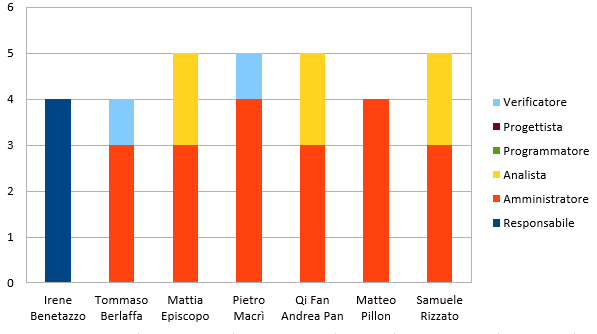
\includegraphics{images/consuntivo/RTB-documentale-ore.png}
    \caption{RTB-Baseline documentale - consuntivo ripartizione oraria}
\end{figure}

\paragraph{Consuntivo Economico}
\begin{center}
	\renewcommand{\arraystretch}{1.8} %aumento ampiezza righe
	\begin{tabular}{ |m{6em}|c|c|c|c|c|c|c| }
	\hline
	\textbf{Ruolo} & \textbf{Re} & \textbf{Am} &  \textbf{An} &  \textbf{Pt} &  \textbf{Pg} &  \textbf{Ve} &  \textbf{Totale}\\
    \hline
    Totale ore & 4 & 20 & 6 & 0 & 0 & 2 & \textbf{32}\\
    \hline
    Costo \euro/h & 30\euro/h & 20\euro/h & 25\euro/h & 25\euro/h & 15\euro/h & 15\euro/h & \\
    \hline
    \textbf{Totale costo} & \textbf{120\euro} & \textbf{400\euro} &  \textbf{150\euro} & \textbf{0\euro} &  \textbf{0\euro} &  \textbf{30\euro} &  \textbf{700\euro} \\
    & (+30\euro) & (-120\euro) & (-75\euro) &  &  & (-15\euro) & (-280\euro) \\
    \hline
	\end{tabular}

    \begin{figure}[H]
       \centering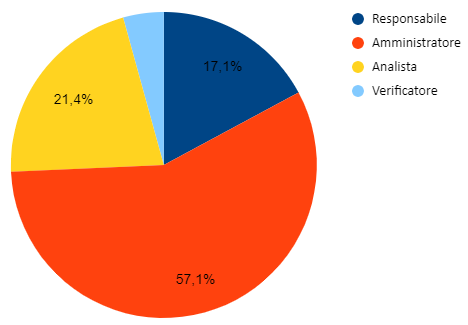
\includegraphics[width=0.6\textwidth, height=0.6\textheight, keepaspectratio]{images/consuntivo/RTB-documentale-costo.png}
       \caption{RTB-Baseline documentale - consuntivo ripartizione economica}
    \end{figure}
\end{center}

\paragraph{Considerazioni} \hfill \break
Erano state preventivate più ore (e giorni) di lavoro per gli amministratori, dato il cospicuo 
numero di pagine dei documenti e si pensava fosse necessario più studio anche per gli analisti.
Quindi questa fase si chiude 7 giorni prima del previsto cioè il 26 Aprile, con un risparmio di 280\euro. 
\begin{center}
	\renewcommand{\arraystretch}{1.8} %aumento ampiezza righe
	\begin{tabular}{ | l |c|c| }
    \hline
    & \textbf{Ore} & \textbf{Costo} \\
	\hline
    \textbf{Consuntivo} & 32 & 700\euro \\
    \hline
    \textbf{Preventivo} & 46 & 980\euro \\
    \hline
    \textbf{Bilancio fase} & -14 & -280\euro \\
    \hline
    \textbf{Bilancio complessivo} & \textbf{-14} & \textbf{-280\euro} \\
    \hline
    \end{tabular}
\end{center}

Di conseguenza si decide di partire subito con la fase successiva: Baseline dei Requisiti di cui inizialmente 
è stata prevista una sola settimana di lavoro, ma dato la grande mole di casi d'uso da identificare e 
analizzare nel progetto probabilmente verrà usato parte del risparmio di questa fase.

\subsubsection{Baseline dei Requisiti}
\paragraph{Consuntivo Orario}
\begin{center}
	\renewcommand{\arraystretch}{1.8}
	\begin{tabular}{ |c|c|c|c|c|c|c|c| }
	\hline
	\textbf{Membro} & \textbf{Re} & \textbf{Am} &  \textbf{An} &  \textbf{Pt} &  \textbf{Pg} &  \textbf{Ve} &  \textbf{Totale}\\
    \hline
    Irene Benetazzo   & - & 3      & 6  (-5) & - & - & 2 & \textbf{11} (-5) \\
    \hline
    Tommaso Berlaffa  & - & 1      & 13      & - & - & - & \textbf{14}      \\
    \hline
    Mattia Episcopo   & - & - (-2) & 13 (+2) & - & - & - & \textbf{13}      \\
    \hline
    Pietro Macrì      & - & 1      & 7  (-6) & - & - & - & \textbf{8} (-6)  \\
    \hline
    Qi Fan Andrea Pan & - & 1      & 7  (-5) & - & - & - & \textbf{8} (-5)  \\
    \hline
    Matteo Pillon     & - & - (-1) & 11 (-2) & - & - & 2 & \textbf{13} (-3) \\
    \hline
    Samuele Rizzato   & 3 & 1      & 5  (-6) & - & - & - & \textbf{9} (-6)  \\
    \hline
    \textbf{Totale ore} & \textbf{3} & \textbf{7} (-3) &  \textbf{62} (-22) &  \textbf{0} &  \textbf{0} &  \textbf{4} &  \textbf{76} (-25)\\
    \hline
	\end{tabular}
\end{center}
\begin{figure}[H]
    \centering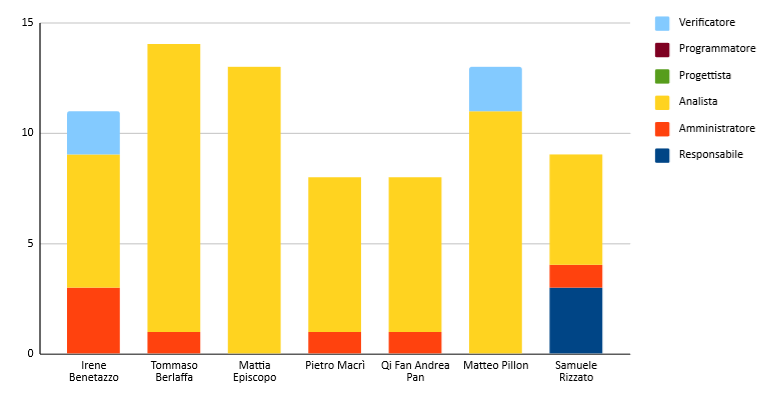
\includegraphics[width=\textwidth, height=\textheight,keepaspectratio]{images/consuntivo/RTB-requisiti-ore.png}
    \caption{RTB-Baseline dei requisiti - consuntivo ripartizione oraria}
\end{figure}

\paragraph{Consuntivo Economico}
\begin{center}
	\renewcommand{\arraystretch}{1.8}
	\begin{tabular}{ |m{6em}|c|c|c|c|c|c|c| }
	\hline
	\textbf{Ruolo} & \textbf{Re} & \textbf{Am} &  \textbf{An} &  \textbf{Pt} &  \textbf{Pg} &  \textbf{Ve} &  \textbf{Totale}\\
    \hline
    Totale ore & 3 & 7 & 62 & 0 & 0 & 4 & \textbf{76}\\
    \hline
    Costo \euro/h & 30\euro/h & 20\euro/h & 25\euro/h & 25\euro/h & 15\euro/h & 15\euro/h & \\
    \hline
    \textbf{Totale costo} & \textbf{90\euro} & \textbf{140\euro} &  \textbf{1550\euro} & \textbf{0\euro} &  \textbf{0\euro} &  \textbf{60\euro} &  \textbf{1840\euro} \\
    &  & (-60\euro) & (-550\euro) &  &  &  & (-610\euro) \\
    \hline
	\end{tabular}

    \begin{figure}[H]
        \centering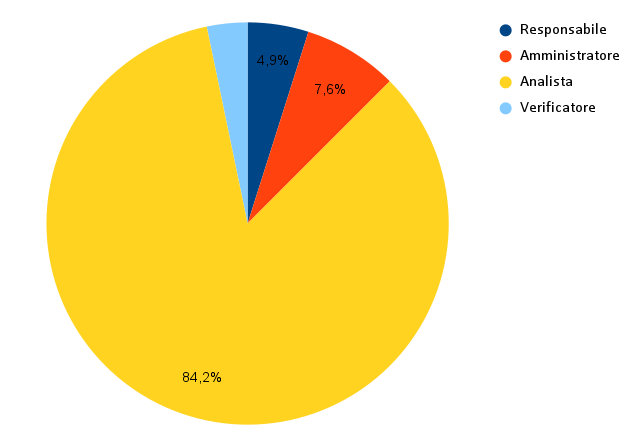
\includegraphics[width=0.7\textwidth, height=0.7\textheight, keepaspectratio]{images/consuntivo/RTB-requisiti-costo.png}
        \caption{RTB-Baseline dei requisiti - consuntivo ripartizione economica}
    \end{figure}
\end{center}

\paragraph{Considerazioni} \hfill \break
Per la maggior parte dei membri del gruppo sono state preventivate più ore di quelle necessarie come analisti in quanto 
si pensava che l'Analisi dei Requisiti avrebbe preso molto tempo per l'identificazione e lo studio dei casi d'uso, inoltre è stata
fatta una sovrastima delle ore da amministratore poiché il team si è dedicato di più all'Analisi dei Requisiti 
che all'aggiornamento dei vari documenti.

\begin{center}
	\renewcommand{\arraystretch}{1.8}
	\begin{tabular}{ | l |c|c| }
    \hline
    & \textbf{Ore} & \textbf{Costo} \\
	\hline
    \textbf{Consuntivo} & 76 & 1840\euro \\
    \hline
    \textbf{Preventivo} & 101 & 2450\euro \\
    \hline
    \textbf{Bilancio fase} & -25 & -610\euro \\
    \hline
    \textbf{Bilancio complessivo} & \textbf{-39} & \textbf{-890\euro} \\
    \hline
    \end{tabular}
\end{center}
In conclusione la fase Baseline dei Requisiti termina il 2022-05-09 come prestabilito con un risparmio, relativo
alla fase, di 610€.

\subsubsection{Baseline delle Tecnologie}
\paragraph{Consuntivo Orario}
\begin{center}
	\renewcommand{\arraystretch}{1.8}
	\begin{tabular}{ |c|c|c|c|c|c|c|c| }
	\hline
	\textbf{Membro} & \textbf{Re} & \textbf{Am} &  \textbf{An} &  \textbf{Pt} &  \textbf{Pg} &  \textbf{Ve} &  \textbf{Totale}\\
    \hline
    Irene Benetazzo   & - & 8 & - & - & 2 & 2 & \textbf{12} \\
    \hline
    Tommaso Berlaffa  & - & - & - & 7 & 3 & -(-2) & \textbf{10} \\
    \hline
    Mattia Episcopo   & 1 & - & - & 8 & 3 & - & \textbf{12} \\
    \hline
    Pietro Macrì      & 1 & 1 & - & 7 & 3 & 2(+2) & \textbf{14} \\
    \hline
    Qi Fan Andrea Pan & 3 & 2 & - & 4 & 3 & - & \textbf{12} \\
    \hline
    Matteo Pillon     & - & - & - & 7 & 3 & 2 & \textbf{12} \\
    \hline
    Samuele Rizzato   & 1 & 5 & 2 & - & 2 & 2 & \textbf{12} \\
    \hline
    \textbf{Totale ore} & \textbf{6} & \textbf{16} &  \textbf{2} &  \textbf{33} &  \textbf{19} &  \textbf{8} &  \textbf{84}\\
    \hline
	\end{tabular}
\end{center}
\begin{figure}[H]
    \centering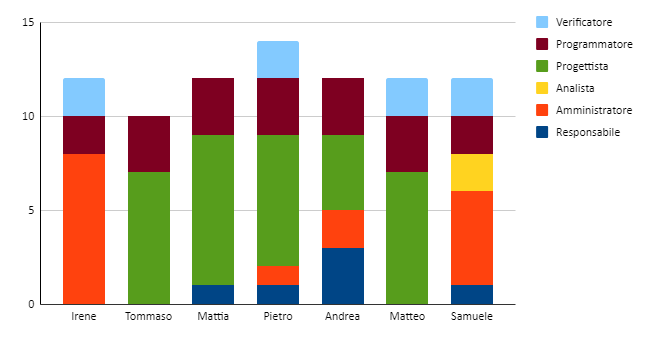
\includegraphics[width=\textwidth, height=\textheight,keepaspectratio]{images/consuntivo/RTB-tecnologico-ore.png}
    \caption{RTB-Baseline delle tecnologie - consuntivo ripartizione oraria}
\end{figure}

\paragraph{Consuntivo Economico}
\begin{center}
	\renewcommand{\arraystretch}{1.8}
	\begin{tabular}{ |m{6em}|c|c|c|c|c|c|c| }
	\hline
	\textbf{Ruolo} & \textbf{Re} & \textbf{Am} &  \textbf{An} &  \textbf{Pt} &  \textbf{Pg} &  \textbf{Ve} &  \textbf{Totale}\\
    \hline
    Totale ore & 6 & 16 & 2 & 33 & 19 & 8 & \textbf{84}\\
    \hline
    Costo \euro/h & 30\euro/h & 20\euro/h & 25\euro/h & 25\euro/h & 15\euro/h & 15\euro/h & \\
    \hline
    \textbf{Totale costo} & \textbf{180\euro} & \textbf{320\euro} &  \textbf{50\euro} &  \textbf{825\euro} &  \textbf{285\euro} &  \textbf{120\euro} &  \textbf{1780\euro}\\
    \hline
	\end{tabular}
    \begin{figure}[H]
        \centering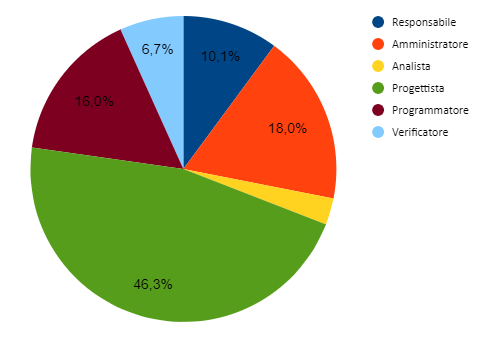
\includegraphics[width=0.7\textwidth, height=0.7\textheight, keepaspectratio]{images/consuntivo/RTB-tecnologico-costo.png}
        \caption{RTB-Baseline delle tecnologie - consuntivo ripartizione economica}
    \end{figure}
\end{center}

\paragraph{Considerazioni} \hfill \break
Durante questa macrofase a livello economico c'è stato un risparmio di ore e costi, anche se a livello temporale è stata necessaria una settimana in più.
Il motivo principale è stato lo studio delle tecnologie necessarie per il PoC, essendo nuove per i membri del gruppo, le ore di studio personale non sono state conteggiate. \newline
\begin{center}
	\renewcommand{\arraystretch}{1.8}
	\begin{tabular}{ | l |c|c| }
    \hline
    & \textbf{Ore} & \textbf{Costo} \\
	\hline
    \textbf{Consuntivo} & 84 & 1780\euro \\
    \hline
    \textbf{Preventivo} & 84 & 1780\euro \\
    \hline
    \textbf{Bilancio fase} & 0 & 0\euro \\
    \hline
    \textbf{Bilancio complessivo} & \textbf{-39} & \textbf{-890\euro} \\
    \hline
    \end{tabular}
\end{center}
In conclusione la fase Baseline delle Tecnologie termina il 2022-05-31.


\subsubsection{Complessivo RTB}
\paragraph{Consuntivo Orario}
\begin{center}
	\renewcommand{\arraystretch}{1.8}
	\begin{tabular}{ |c|c|c|c|c|c|c|c| }
	\hline
	\textbf{Membro} & \textbf{Re} & \textbf{Am} &  \textbf{An} &  \textbf{Pt} &  \textbf{Pg} &  \textbf{Ve} &  \textbf{Totale}\\
    \hline
    Irene Benetazzo   & 4 & 11 & 6 & - & 2 & 4 & \textbf{27} \\
    \hline
    Tommaso Berlaffa  & - & 4 & 13 & 7 & 3 & 1 & \textbf{28} \\
    \hline
    Mattia Episcopo   & 1 & 3 & 15 & 8 & 3 & - & \textbf{30} \\
    \hline
    Pietro Macrì      & 1 & 6 & 7 & 7 & 3 & 3 & \textbf{27} \\
    \hline
    Qi Fan Andrea Pan & 3 & 6 & 9 & 4 & 3 & - & \textbf{25} \\
    \hline
    Matteo Pillon     & - & 4 & 11 & 7 & 3 & 4 & \textbf{29} \\
    \hline
    Samuele Rizzato   & 4 & 9 & 9 & - & 2 & 2 & \textbf{26} \\
    \hline
    \textbf{Totale ore} & \textbf{13} & \textbf{43} &  \textbf{70} &  \textbf{33} &  \textbf{19} &  \textbf{14} &  \textbf{192}\\
    \hline
	\end{tabular}
\end{center}
\begin{figure}[H]
    \centering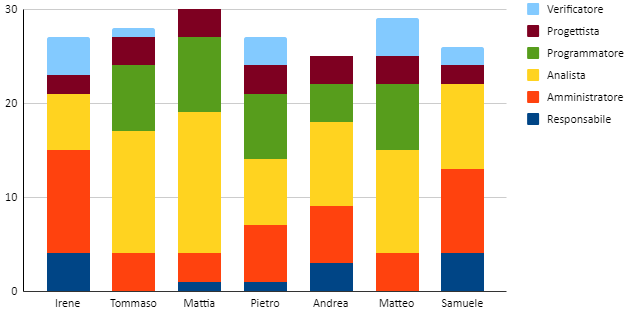
\includegraphics[width=\textwidth, height=\textheight,keepaspectratio]{images/consuntivo/RTB-ore.png}
    \caption{Totale RTB - consuntivo ripartizione oraria}
\end{figure}

\paragraph{Consuntivo Economico}
\begin{center}
	\renewcommand{\arraystretch}{1.8}
	\begin{tabular}{ |m{6em}|c|c|c|c|c|c|c| }
	\hline
	\textbf{Ruolo} & \textbf{Re} & \textbf{Am} &  \textbf{An} &  \textbf{Pt} &  \textbf{Pg} &  \textbf{Ve} &  \textbf{Totale}\\
    \hline
    Totale ore & 13 & 43 & 70 & 33 & 19 & 14 & \textbf{192}\\
    \hline
    Costo \euro/h & 30\euro/h & 20\euro/h & 25\euro/h & 25\euro/h & 15\euro/h & 15\euro/h & \\
    \hline
    \textbf{Totale costo} & \textbf{390\euro} & \textbf{860\euro} &  \textbf{1750\euro} &  \textbf{825\euro} &  \textbf{285\euro} &  \textbf{210\euro} &  \textbf{4320\euro}\\
    \hline
	\end{tabular}

    \begin{figure}[H]
        \centering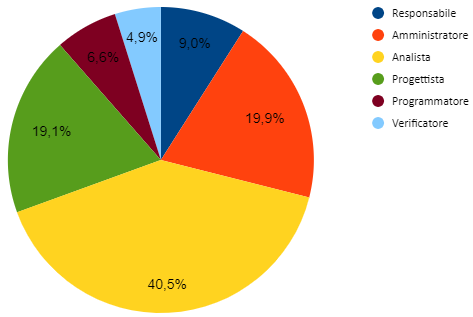
\includegraphics[width=0.7\textwidth, height=0.7\textheight, keepaspectratio]{images/consuntivo/RTB-costo.png}
        \caption{Totale RTB - consuntivo ripartizione economica}
    \end{figure}
\end{center}

\paragraph{Considerazioni} \hfill \break
\begin{center}
	\renewcommand{\arraystretch}{1.8}
	\begin{tabular}{ | l |c|c| }
    \hline
    & \textbf{Ore} & \textbf{Costo} \\
	\hline
    \textbf{Consuntivo} & 192 & 4320\euro \\
    \hline
    \textbf{Preventivo} & 231 & 5210\euro \\
    \hline
    \textbf{Bilancio} & \textbf{-39} & \textbf{-890\euro} \\
    \hline
    \end{tabular}
\end{center}
In conclusione la macrofase Requirements Tecnology Baseline iniziata il 2022-04-19 termina il 2022-06-01 con un ritardo di 9 giorni e un risparmio di 890\euro.

\paragraph{Preventivo a Finire} \hfill \break
Considerato l'avanzo complessivo di 39 ore oltre ad una non corretta distribuzione delle ore nei specifici ruoli, nel documento \emph{Candidatura.pdf}, si è deciso di ridistribuire la pianificazione delle ore nei ruoli:
\begin{center}
	\renewcommand{\arraystretch}{1.8}
	\begin{tabular}{ | l |c|c|c| }
    \hline
    \textbf{Ruolo} & \textbf{Preventivo attuale} & \textbf{Preventivo iniziale}  & \textbf{Differenza economica}\\
	\hline
    \textbf{Responsabile} & 40 & 40 & 0\euro \\
    \hline
    \textbf{Amministratore} & 90 & 100 & -200\euro \\
    \hline
    \textbf{Analista} & 70 & 100 & -750\euro \\
    \hline
    \textbf{Progettista} & 170 & 160 & 250\euro \\
    \hline
    \textbf{Programmatore} & 190 & 160 & 450\euro \\
    \hline
    \textbf{Verificatore} & 140 & 140 & 0\euro \\
    \hline
    \textbf{Totale} & \textbf{700} & \textbf{700} & \textbf{-250\euro} \\
    \hline
    \end{tabular}
\end{center}
Non è cambiato il numero complessivo di ore ma la distribuzione interna e data la differenza di prezzo tra i vari ruoli, ciò porta ad un risparmio di 250 \euro rispetto al preventivo iniziale. \newline
Il preventivo della macrofase Product Baseline (\$5.2) è stato stilato basandosi sul preventivo attuale.

\subsubsection{Fase Aggiuntiva per Sistemazione Documenti}
\paragraph{Consuntivo Orario}
\begin{center}
	\renewcommand{\arraystretch}{1.8}
	\begin{tabular}{ |c|c|c|c|c|c|c|c| }
	\hline
	\textbf{Membro} & \textbf{Re} & \textbf{Am} &  \textbf{An} &  \textbf{Pt} &  \textbf{Pg} &  \textbf{Ve} &  \textbf{Totale}\\
    \hline
    Irene Benetazzo   & - & 1 & - & - & - & 1 & \textbf{2} \\
    \hline
    Tommaso Berlaffa  & - & - & 1 & - & - & - & \textbf{1} \\
    \hline
    Mattia Episcopo   & - & - & 1 & - & - & - & \textbf{1} \\
    \hline
    Pietro Macrì      & - & - & - & - & - & 1 & \textbf{1} \\
    \hline
    Qi Fan Andrea Pan & - & - & 1 & - & - & - & \textbf{1} \\
    \hline
    Matteo Pillon     & 2 & - & 1 & - & - & - & \textbf{3} \\
    \hline
    Samuele Rizzato   & 1 & 1 & - & - & - & - & \textbf{2} \\
    \hline
    \textbf{Totale ore} & \textbf{3} & \textbf{2} &  \textbf{4} &  \textbf{0} &  \textbf{0} &  \textbf{2} &  \textbf{11}\\
    \hline
	\end{tabular}
\end{center}

\begin{figure}[H]
    \centering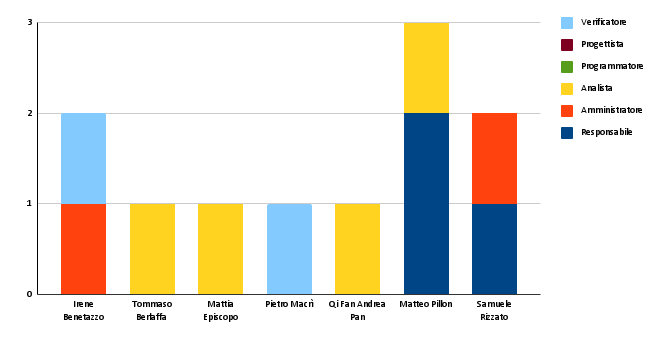
\includegraphics[width=\textwidth, height=\textheight,keepaspectratio]{images/consuntivo/RTB-fase-aggiuntiva-ore.png}
    \caption{RTB-Fase aggiuntiva - consuntivo ripartizione oraria}
\end{figure}

\paragraph{Consuntivo Economico}
\begin{center}
	\renewcommand{\arraystretch}{1.8}
	\begin{tabular}{ |m{6em}|c|c|c|c|c|c|c| }
	\hline
	\textbf{Ruolo} & \textbf{Re} & \textbf{Am} &  \textbf{An} &  \textbf{Pt} &  \textbf{Pg} &  \textbf{Ve} &  \textbf{Totale}\\
    \hline
    Totale ore & 3 & 2 & 4 & 0 & 0 & 2 & \textbf{11}\\
    \hline
    Costo \euro/h & 30\euro/h & 20\euro/h & 25\euro/h & 25\euro/h & 15\euro/h & 15\euro/h & \\
    \hline
    \textbf{Totale costo} & \textbf{90\euro} & \textbf{40\euro} &  \textbf{100\euro} &  \textbf{0\euro} &  \textbf{0\euro} &  \textbf{30\euro} &  \textbf{260\euro}\\
    \hline
	\end{tabular}
    \begin{figure}[H]
        \centering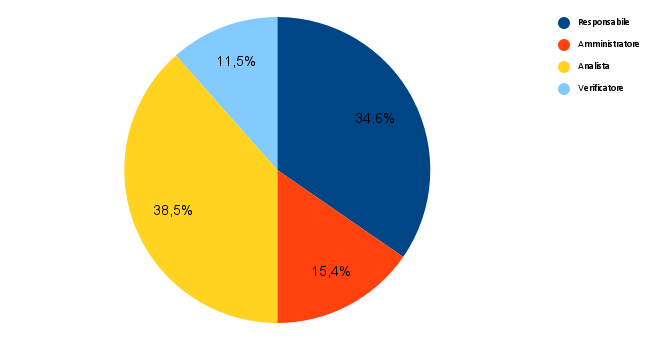
\includegraphics[width=0.7\textwidth, height=0.7\textheight, keepaspectratio]{images/consuntivo/RTB-fase-aggiuntiva-costo.png}
        \caption{RTB-Fase aggiuntiva - consuntivo ripartizione economica}
    \end{figure}
\end{center}

\paragraph{Considerazioni} \hfill \break
Queste 11 ore sono tutte oltre il preventivo a livello numerico mentre a livello economico si riescono a compensare con i 250\euro risparmiati nella ripianificazione eseguita al termine della scorsa fase.
Quindi attualmente con il bilancio si è in negativo di soli 10\euro. 
\newline In seguito all'aggiunta di questa fase, il gruppo prende atto che la fase successiva slitterà di almeno una settimana, a causa della necessità di sistemazione dei documenti e succesivo inoltro per la verifica. 